\documentclass[acmtog]{acmart}
\usepackage{graphicx}
\usepackage{subfigure}
\usepackage{natbib}
\usepackage{listings}
\usepackage{bm}
\usepackage{amsmath}

\definecolor{blve}{rgb}{0.3372549 , 0.61176471, 0.83921569}
\definecolor{gr33n}{rgb}{0.29019608, 0.7372549, 0.64705882}
\makeatletter
\lst@InstallKeywords k{class}{classstyle}\slshape{classstyle}{}ld
\makeatother
\lstset{language=C++,
	basicstyle=\ttfamily,
	keywordstyle=\radiance{blve}\ttfamily,
	stringstyle=\radiance{red}\ttfamily,
	commentstyle=\radiance{magenta}\ttfamily,
	morecomment=[l][\radiance{magenta}]{\#},
	classstyle = \bfseries\radiance{gr33n},
	tabsize=2
}
\lstset{basicstyle=\ttfamily}

% Title portion
\title{Assignment 4: {Global Illumination}}

\author{Name:\quad Hidden \\ student number:\ Hidden
\\email:\quad Hidden@shanghaitech.edu.cn}

% Document starts
\begin{document}
\maketitle

\vspace*{2 ex}

\section{Introduction}

In this assignment, the following `must' tasks are implemented.

\begin{itemize}
	\item Path tracing with Monte Carlo integration, direct + indirect lighting.
	\item Ideal diffuse BRDF and square area light source
	\item Acceleration structure: BVH
\end{itemize}

and the following `bonus' tasks are implemented.

\begin{itemize}
	\item Ideal specular BRDF
	\item Advanced BVH with higher performance, including
	\begin{itemize}
		\item Global BVH
		\item Morton code
		\item Linearized BVH
	\end{itemize} 
\end{itemize}

\section{Implementation Details}

\subsection{Path tracing with Monte-Carlo integration}

\begin{center}
	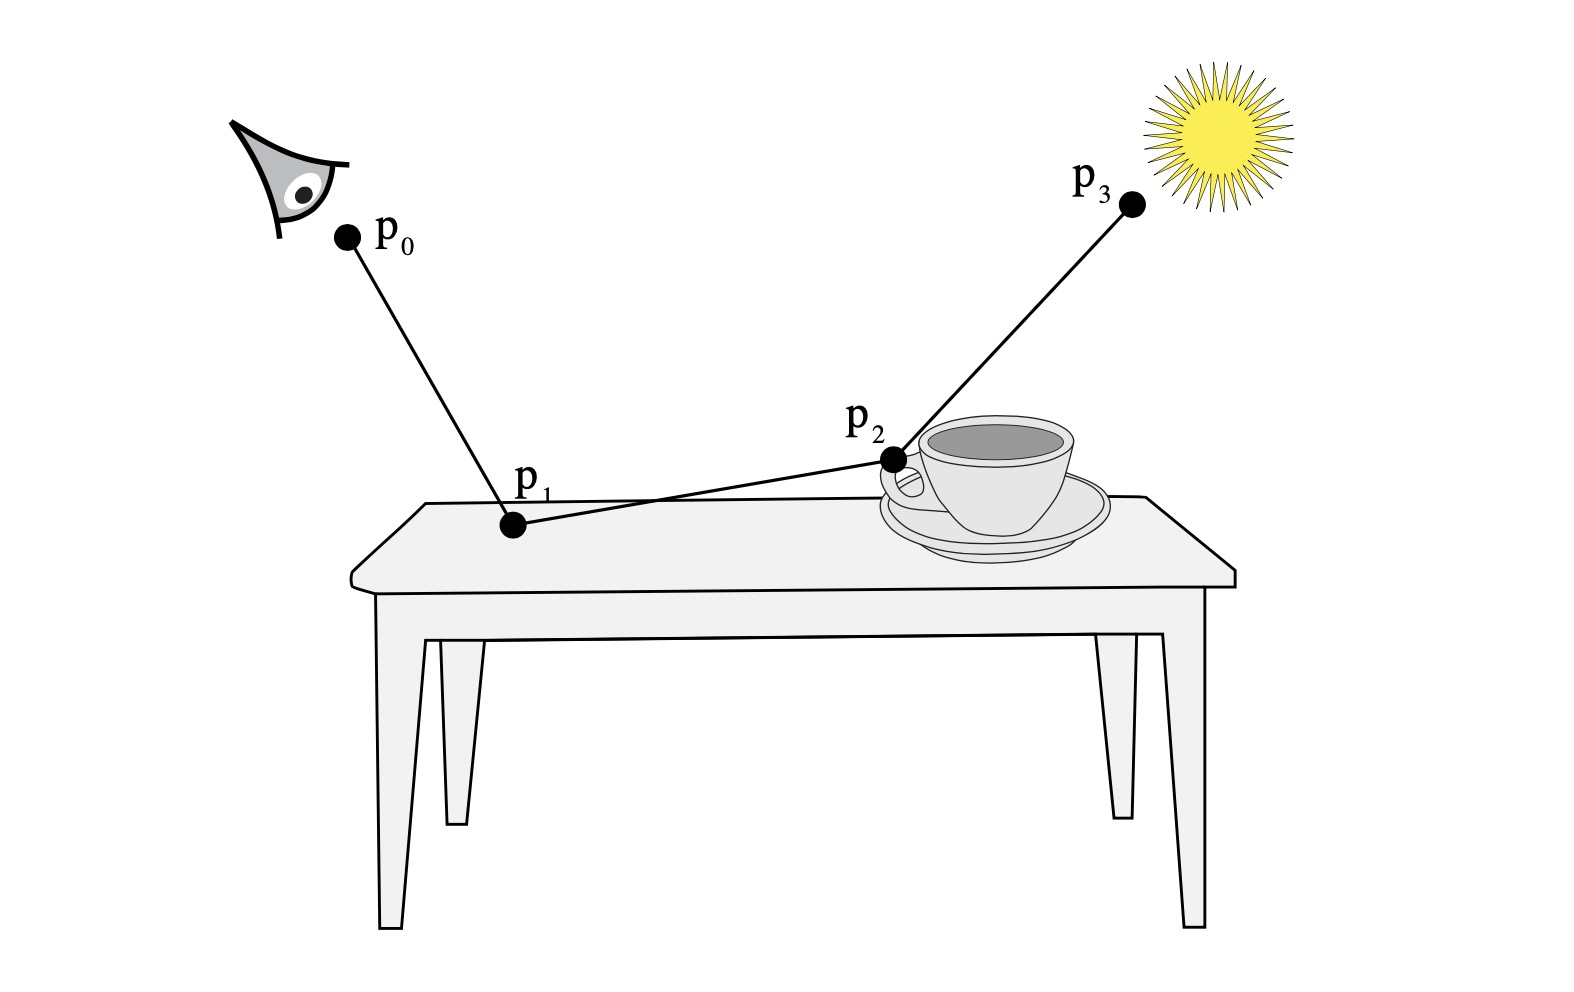
\includegraphics[width=0.4\textwidth]{pictures/path-sampling.jpg}
\end{center}

To calculate radiance of a pixel, we divide the ray's path into two parts: direct lighting and indirect lighting.

\begin{itemize}
	\item \textbf{Direct lighting}:
	
	The direct lighting is calculated by sampling the light source.
	
	\[
		L_0 (x, \omega_o) = \int_{A} L_i(x, \omega_i) f(x, \omega_i, \omega_o)  \frac{\cos \theta \cos \theta'}{\| x' - x \|^2} \mathrm{d}\omega_i
	\]

	where $L_i(x, \omega_i)$ is the radiance of the light source, $f(x, \omega_i, \omega_o)$ is the BSDF of the material, $\omega_i$ and $\omega_o$ are the incoming and outgoing directions, $\theta$ and $\theta'$ are the angles between the normal and the incoming and outgoing directions, respectively. $A$ is the area of the light source.

	By Monte-Carlo integration, we can get the direct lighting as follows:
	\[
		L_0 (x, \omega_o) \approx \frac{1}{N} \sum_{i=1}^{N} L_i(x, \omega_i) f(x, \omega_i, \omega_o)  \frac{\cos \theta \cos \theta'}{\| x' - x \|^2}
	\]

	\item \textbf{Indirect lighting}:
	
	The indirect lighting is calculated by the following rendering equation. We are applying Monte-Carlo cosine-weighted sampling on a hemisphere.

	\[
		\begin{aligned}
			L_0(x, \omega_0) = \sum_{\Omega^+} L_i(x, \omega_i) f_r(x, \omega_i, \omega_o) \cos\theta \mathrm{d} \omega_i\\
			\approx \frac{1}{N} \sum_{i=1}^{N} \frac{L_i(x, \omega_i) f_r(x, \omega_i, \omega_o)(n\cdot \omega_i)}{p(\omega_i)}
		\end{aligned}
	\]

	where $L_i(x, \omega_i)$ is the radiance of the light source, $f_r(x, \omega_i, \omega_o)$ is the BSDF of the material, $\omega_i$ and $\omega_o$ are the incoming and outgoing directions, $\theta$ is the angle between the normal and the incoming direction, $n\cdot \omega_i$ is the cosine of the angle between the normal and the incoming direction, $p(\omega_i)$ is the probability density function of the incoming direction. $\Omega^+$ is the hemisphere above the surface.


\end{itemize}

Then for each ray, we perform Monte-Carlo path tracing with the following recursive procedure. 

\begin{enumerate}
	\item We first check the recursion depth limit. If limit exceeded, return zero.
	\item If a ray hits a light, return light emission.
	\item If a ray hits an object (geometry), sample the light and get the direct lighting. Then shoot another ray to recursively compute indirect light.
	\item Check if the direct lighting and indirect lighting are valid, that is, not NaN and not Infinity. If invalid, change it to Zero.
	\item Return direct lighting and indirect lighting. 
\end{enumerate}


To improve efficiency, instead of sampling multiple incident rays on the intersection point, we only sample one incident ray and then trace it to the next intersection point. We greatly increase the sample rate in one pixel to make the scene more smooth and realistic. 




\subsection{BSDF}

BSDF, the Bidirectional Scattering Distribution Function, is a function that describes the distribution of light reflected by a surface. It is a function of the incident and outgoing directions. It can used to calculate the direct lighting. In this assignment, ideal diffusion and ideal specular (mirror) are implemented. We will explain these two materials in the following section.

\newpage

\begin{itemize}
	\item \textbf{Ideal diffusion BSDF}:
	
	\begin{center}
		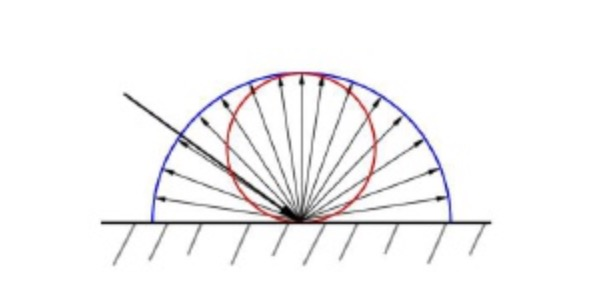
\includegraphics[width=0.4\textwidth]{pictures/ideal-diffuse.jpg}
	\end{center}

	For ideal diffusion BRDF, we use cos-weighted sampling. First we generate two uniform samples in $[0.0, 1.0]$, namely $(x, y)$.

	Then we transform the above $(x,y)$ to $(r, \theta_1)$.

	\[\begin{cases}
		r = \sqrt{x_1}\\
		\theta_1 = 2\pi y_1
	\end{cases}\]

	Then we project it to the unit hemisphere. Note that any point on a sphere can be represented by $(\theta, \phi)$ using the following parameter expression 
	\[\begin{cases}
		x = \sin \theta \cos \phi\\
		y = \sin \theta \sin \phi\\
		z = \cos \theta
	\end{cases}\]

	We get the value of $\theta$ and $\phi$ by \[\begin{cases}
		\sin \theta = r = \sqrt{x_1}\\
		\phi = \theta_1 = 2\pi y_1
	\end{cases}\]

	Finally we convert it from the local (object-centered) local coordinate to the world coordinate using the normal vector.

	Then we get the sampled incoming ray. The PDF is equal to \[
		\frac{\cos \theta}{\pi}
	\]

	\item \textbf{Ideal Specular BSDF}:
	
	\begin{center}
		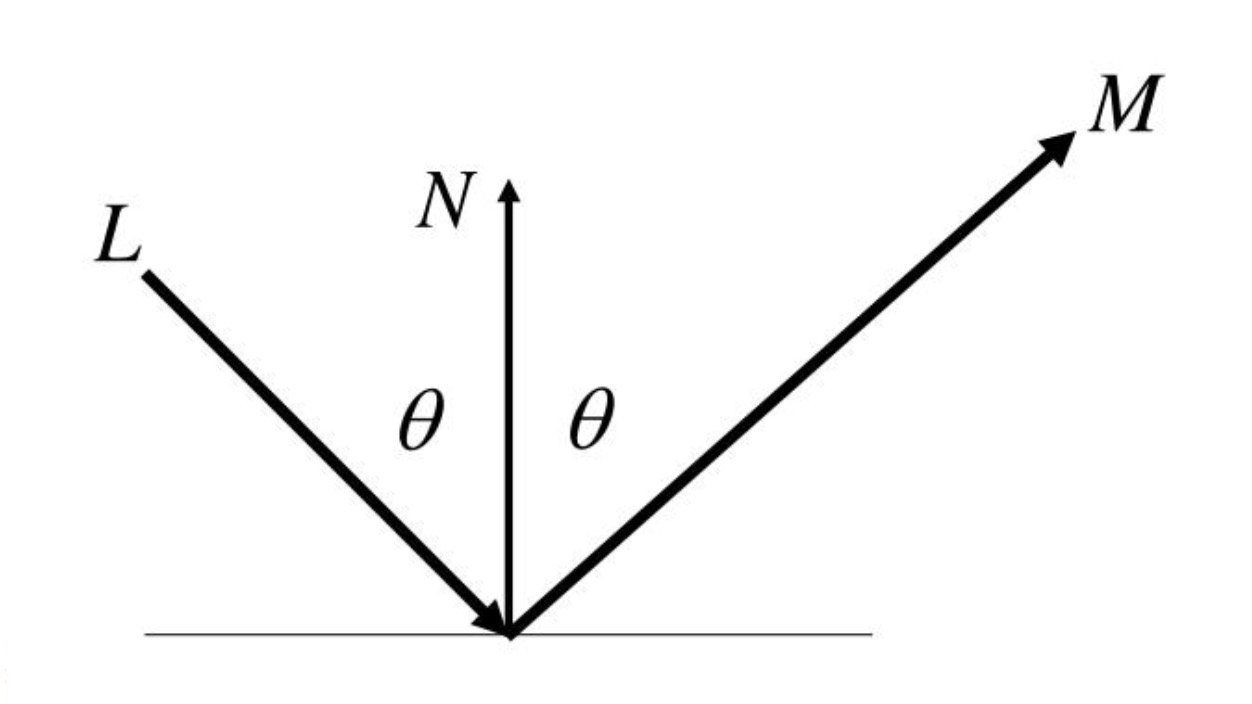
\includegraphics[width=0.4\textwidth]{pictures/ideal-specular.jpg}
	\end{center}
	
	Ideal specular is comparatively easy. We simply sample the reflect light, which should have a pdf of $1$. The reflect direction is given by \[
		w_i = 2(w_0 \cdot n) n - w_0
	\]


\end{itemize}


\subsection{Acceleration structure: BVH}

\begin{itemize}
	\item \textbf{BVH introduction}:


The BVH, Bounding Volumn Hierarchy, is a data structure to store the triangles which can help efficiently do the ray-triangle intersection test. 
The BVH is a binary tree, where each node is an axis-aligned bounding box (aka. AABB). 
The root node is the bounding box of the whole scene. 
The left and right child of a node are the bounding boxes of the left and right part of the scene. 
Each leaf node is the bounding box containing one or only a small number of a triangle. 

An intuitive explanation of BVH is shown in the following picture (source: https://developer.nvidia.com/blog/thinking-parallel-part-ii-tree-traversal-gpu/).

\begin{center}
	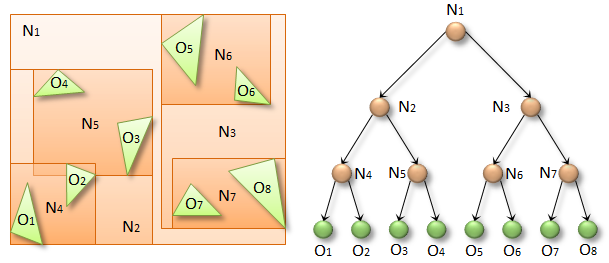
\includegraphics[width=0.4\textwidth]{pictures/bvh.png}
\end{center}

	\item \textbf{BVH construction}:

In this assignment, we construct a BVH using morton code to make it more cache-friendly, thus improving performance. 

The morton code of a point is a 32-bit integer, which is a combination of the binary representation of the x, y, z coordinates of the point. For each triangle, its morton code is the morton code of its gravity center point. 
Before calculation of the morton code, we put every triangle in a large AABB and normalize the coordinates of the triangles to $[0, 1]^3$. 



After calculating the morton code of every triangle, we sort the triangles according to their morton code. 
In this way, when we can traverse triangles in a Z-order manner, making triangles close to each other in the scene also close to each other in the BVH, which also means that they are close in memory. 

\begin{center}
	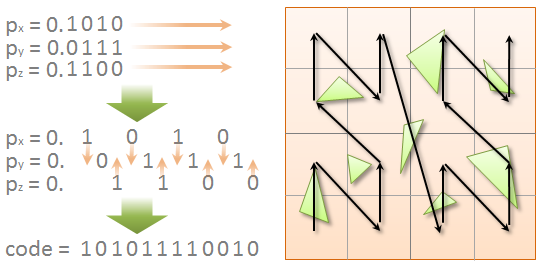
\includegraphics[width=0.4\textwidth]{pictures/morton-code-and-z-curve.png}

	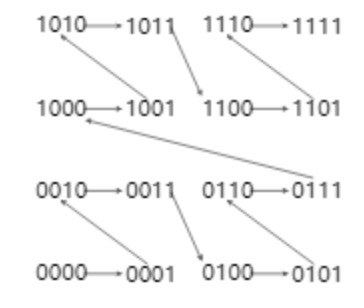
\includegraphics[width=0.2\textwidth]{pictures/morton-z.jpg}
\end{center}

Then we can start constructing BVH.

The BVH is constructed by recursively splitting the bounding box into two parts. 
The split point is the highest digit of where the Morton code changes.
For example, if the Morton code of a triangle is 000000000, and the Morton code of the next triangle is 01000000, then the split point is the 7st digit.
After splitting the bounding box, we recursively construct the left and right child of the node, until each leaf node contains only at most 8 triangles.

\begin{center}
	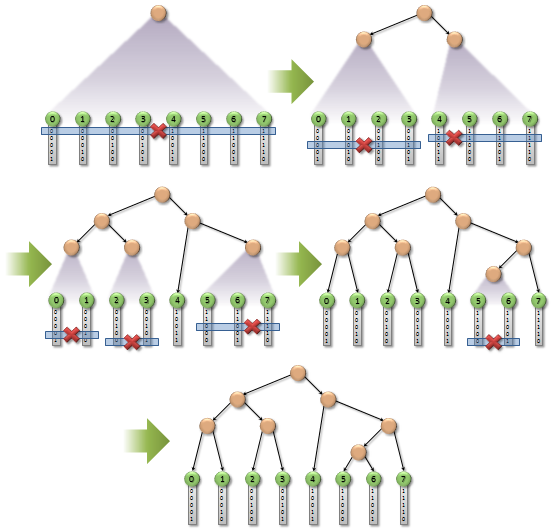
\includegraphics[width=0.4\textwidth]{pictures/top-down-generation.png}
\end{center}

However, the above method may still not be cache-friendly because the triangles are actually pointers. Although pointers are consequtive, the address they are referencing are not consequtive. 

To address this problem, we make the BVH a linearized structure by DFS traversal and store nodes in a one-dimensional array. For internal nodes, we only store the AABB (bounding box) and the index of the right child, since the left child is exactly to the right of it in DFS order. For leaf nodes, we only store the index of the first and last triangle it contains. In this way, a more cache-friendly tree can be built.


\begin{center}
	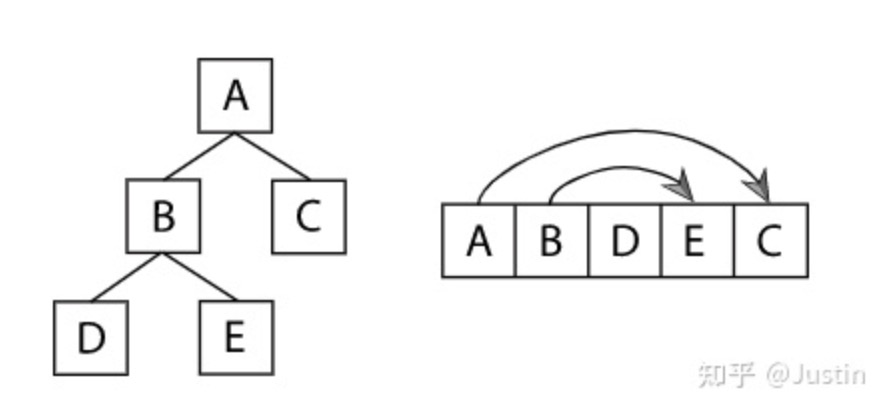
\includegraphics[width=0.4\textwidth]{pictures/linear-bvh-memory.jpg}
\end{center}

	\item \textbf{BVH traversal and intersection test}:

To detect whether a ray intersects with a triangle, we first check whether the ray intersects with the bounding box of the triangle. If it does, we check whether the ray intersects with the triangle. If it does, we update the intersection point and the normal of the triangle.

For intersection test, we first check whether the ray hits the AABB. If it does not, we can directly return false. 

If it hits the AABB, then we recursively check whether it hits the left and right child of the AABB. When the ray hits the left node, we check whether it hits the triangles inside it in the ordinary way. The recursive method makes intersection test possible, and BVH tree makes it much faster.


\end{itemize}

\newpage

\section{Results}


\subsection{Small scene}

The rendered result of the default small scene is shown below. No acceleration structure used (we just use the naive method to traverse all the triangles).

Config file: \verb|configs/simple.json|

Performance: Takes 90 seconds on AMD Ryzen7 5800X (8 cores, 16 threads, 4.51GHz, PBO off)

\begin{center}
	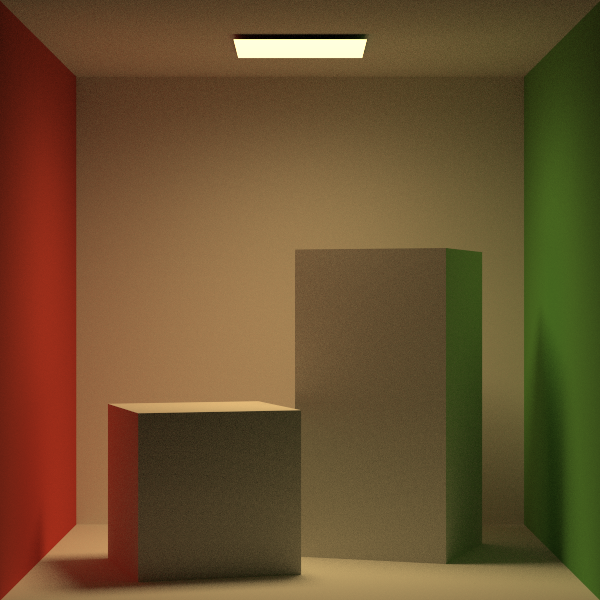
\includegraphics[width=0.4\textwidth]{rendered-results/result-small-scene-bvh.png}
\end{center}

\subsection{Small scene with ideal specular BSDF}

We change the material of the large cube to ideal specular BSDF. The result is shown in the following picture.

Config file: configs/simple-mirror.json

Performance: Takes 89 seconds on AMD R7 5800X

\begin{center}
	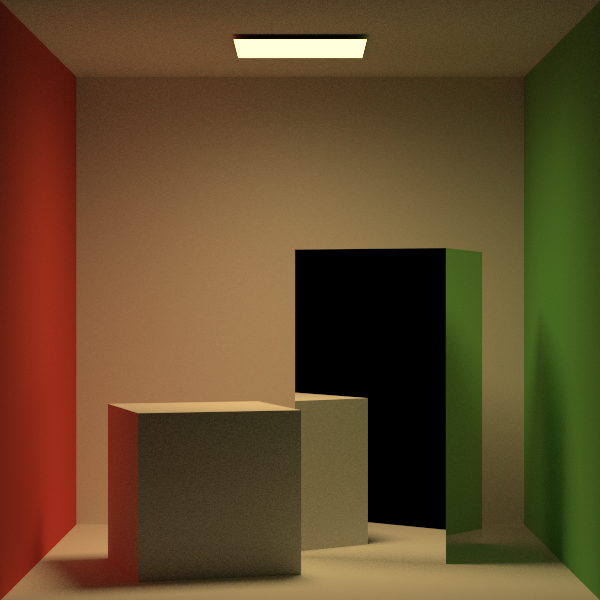
\includegraphics[width=0.4\textwidth]{rendered-results/result-small-scene-bvh-mirror-90s.png}
\end{center}


\newpage

\subsection{Large scene with BVH acceleration}

The large scene contains a bunny object and a dragon object. Together they contain 441391 vertices and 878775 triangle faces. So we must rely on acceleration structure to get the result. With linearized BVH, the render result is shown below.

Config file: \verb|configs/large_mesh.json|

Performance: Takes 139 seconds on AMD R7 5800X 
\begin{center}
	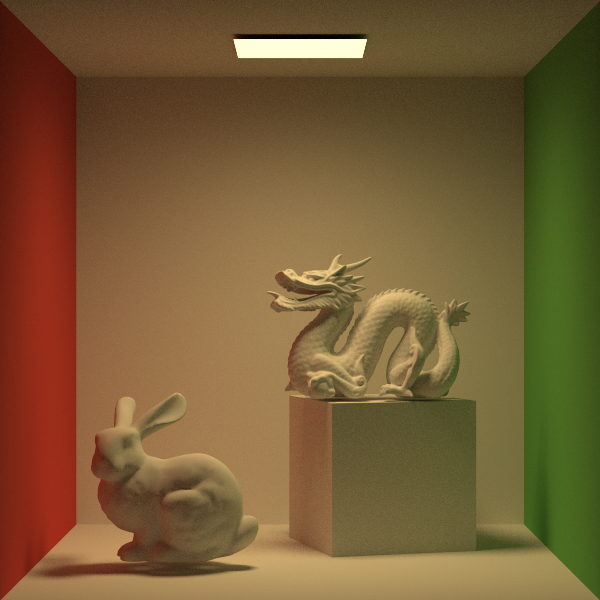
\includegraphics[width=0.4\textwidth]{rendered-results/result-large-scene-bvh-178s.png}
\end{center}



\end{document}
